% Options for packages loaded elsewhere
\PassOptionsToPackage{unicode}{hyperref}
\PassOptionsToPackage{hyphens}{url}
%
\documentclass[
]{article}
\usepackage{amsmath,amssymb}
\usepackage{iftex}
\ifPDFTeX
  \usepackage[T1]{fontenc}
  \usepackage[utf8]{inputenc}
  \usepackage{textcomp} % provide euro and other symbols
\else % if luatex or xetex
  \usepackage{unicode-math} % this also loads fontspec
  \defaultfontfeatures{Scale=MatchLowercase}
  \defaultfontfeatures[\rmfamily]{Ligatures=TeX,Scale=1}
\fi
\usepackage{lmodern}
\ifPDFTeX\else
  % xetex/luatex font selection
\fi
% Use upquote if available, for straight quotes in verbatim environments
\IfFileExists{upquote.sty}{\usepackage{upquote}}{}
\IfFileExists{microtype.sty}{% use microtype if available
  \usepackage[]{microtype}
  \UseMicrotypeSet[protrusion]{basicmath} % disable protrusion for tt fonts
}{}
\makeatletter
\@ifundefined{KOMAClassName}{% if non-KOMA class
  \IfFileExists{parskip.sty}{%
    \usepackage{parskip}
  }{% else
    \setlength{\parindent}{0pt}
    \setlength{\parskip}{6pt plus 2pt minus 1pt}}
}{% if KOMA class
  \KOMAoptions{parskip=half}}
\makeatother
\usepackage{xcolor}
\usepackage[margin=1in]{geometry}
\usepackage{color}
\usepackage{fancyvrb}
\newcommand{\VerbBar}{|}
\newcommand{\VERB}{\Verb[commandchars=\\\{\}]}
\DefineVerbatimEnvironment{Highlighting}{Verbatim}{commandchars=\\\{\}}
% Add ',fontsize=\small' for more characters per line
\usepackage{framed}
\definecolor{shadecolor}{RGB}{248,248,248}
\newenvironment{Shaded}{\begin{snugshade}}{\end{snugshade}}
\newcommand{\AlertTok}[1]{\textcolor[rgb]{0.94,0.16,0.16}{#1}}
\newcommand{\AnnotationTok}[1]{\textcolor[rgb]{0.56,0.35,0.01}{\textbf{\textit{#1}}}}
\newcommand{\AttributeTok}[1]{\textcolor[rgb]{0.13,0.29,0.53}{#1}}
\newcommand{\BaseNTok}[1]{\textcolor[rgb]{0.00,0.00,0.81}{#1}}
\newcommand{\BuiltInTok}[1]{#1}
\newcommand{\CharTok}[1]{\textcolor[rgb]{0.31,0.60,0.02}{#1}}
\newcommand{\CommentTok}[1]{\textcolor[rgb]{0.56,0.35,0.01}{\textit{#1}}}
\newcommand{\CommentVarTok}[1]{\textcolor[rgb]{0.56,0.35,0.01}{\textbf{\textit{#1}}}}
\newcommand{\ConstantTok}[1]{\textcolor[rgb]{0.56,0.35,0.01}{#1}}
\newcommand{\ControlFlowTok}[1]{\textcolor[rgb]{0.13,0.29,0.53}{\textbf{#1}}}
\newcommand{\DataTypeTok}[1]{\textcolor[rgb]{0.13,0.29,0.53}{#1}}
\newcommand{\DecValTok}[1]{\textcolor[rgb]{0.00,0.00,0.81}{#1}}
\newcommand{\DocumentationTok}[1]{\textcolor[rgb]{0.56,0.35,0.01}{\textbf{\textit{#1}}}}
\newcommand{\ErrorTok}[1]{\textcolor[rgb]{0.64,0.00,0.00}{\textbf{#1}}}
\newcommand{\ExtensionTok}[1]{#1}
\newcommand{\FloatTok}[1]{\textcolor[rgb]{0.00,0.00,0.81}{#1}}
\newcommand{\FunctionTok}[1]{\textcolor[rgb]{0.13,0.29,0.53}{\textbf{#1}}}
\newcommand{\ImportTok}[1]{#1}
\newcommand{\InformationTok}[1]{\textcolor[rgb]{0.56,0.35,0.01}{\textbf{\textit{#1}}}}
\newcommand{\KeywordTok}[1]{\textcolor[rgb]{0.13,0.29,0.53}{\textbf{#1}}}
\newcommand{\NormalTok}[1]{#1}
\newcommand{\OperatorTok}[1]{\textcolor[rgb]{0.81,0.36,0.00}{\textbf{#1}}}
\newcommand{\OtherTok}[1]{\textcolor[rgb]{0.56,0.35,0.01}{#1}}
\newcommand{\PreprocessorTok}[1]{\textcolor[rgb]{0.56,0.35,0.01}{\textit{#1}}}
\newcommand{\RegionMarkerTok}[1]{#1}
\newcommand{\SpecialCharTok}[1]{\textcolor[rgb]{0.81,0.36,0.00}{\textbf{#1}}}
\newcommand{\SpecialStringTok}[1]{\textcolor[rgb]{0.31,0.60,0.02}{#1}}
\newcommand{\StringTok}[1]{\textcolor[rgb]{0.31,0.60,0.02}{#1}}
\newcommand{\VariableTok}[1]{\textcolor[rgb]{0.00,0.00,0.00}{#1}}
\newcommand{\VerbatimStringTok}[1]{\textcolor[rgb]{0.31,0.60,0.02}{#1}}
\newcommand{\WarningTok}[1]{\textcolor[rgb]{0.56,0.35,0.01}{\textbf{\textit{#1}}}}
\usepackage{graphicx}
\makeatletter
\def\maxwidth{\ifdim\Gin@nat@width>\linewidth\linewidth\else\Gin@nat@width\fi}
\def\maxheight{\ifdim\Gin@nat@height>\textheight\textheight\else\Gin@nat@height\fi}
\makeatother
% Scale images if necessary, so that they will not overflow the page
% margins by default, and it is still possible to overwrite the defaults
% using explicit options in \includegraphics[width, height, ...]{}
\setkeys{Gin}{width=\maxwidth,height=\maxheight,keepaspectratio}
% Set default figure placement to htbp
\makeatletter
\def\fps@figure{htbp}
\makeatother
\setlength{\emergencystretch}{3em} % prevent overfull lines
\providecommand{\tightlist}{%
  \setlength{\itemsep}{0pt}\setlength{\parskip}{0pt}}
\setcounter{secnumdepth}{-\maxdimen} % remove section numbering
\ifLuaTeX
  \usepackage{selnolig}  % disable illegal ligatures
\fi
\IfFileExists{bookmark.sty}{\usepackage{bookmark}}{\usepackage{hyperref}}
\IfFileExists{xurl.sty}{\usepackage{xurl}}{} % add URL line breaks if available
\urlstyle{same}
\hypersetup{
  pdftitle={Tarea 1},
  pdfauthor={Maria Carolina Navarro Monge C05513; Tábata Picado Carmona C05961; Jose Pablo Trejos Conejo C07862},
  hidelinks,
  pdfcreator={LaTeX via pandoc}}

\title{Tarea 1}
\author{Maria Carolina Navarro Monge C05513 \and Tábata Picado Carmona
C05961 \and Jose Pablo Trejos Conejo C07862}
\date{}

\begin{document}
\maketitle

\hypertarget{parte-i}{%
\section{Parte I}\label{parte-i}}

\textbf{1.Análisis descriptivo de las variables Cuotas y Salarios con
respecto a la variable Sexo.}

Primeramente, se cargan las librerías , la base de datos y se fija una
semilla para la reproducibilidad de los resultados.

\begin{Shaded}
\begin{Highlighting}[]
\FunctionTok{library}\NormalTok{(knitr)}
\NormalTok{tinytex}\SpecialCharTok{::}\FunctionTok{install\_tinytex}\NormalTok{(}\AttributeTok{force =} \ConstantTok{TRUE}\NormalTok{)}
\FunctionTok{library}\NormalTok{(tidyverse)}
\FunctionTok{library}\NormalTok{(plotly)}
\FunctionTok{library}\NormalTok{(DT)}
\FunctionTok{library}\NormalTok{(univariateML)}
\FunctionTok{library}\NormalTok{(rriskDistributions) }\CommentTok{\#encuentra que distribuciónn de probabilidades es la}
                            \CommentTok{\#que ajusta mejor con una colección de datos.}
                            \CommentTok{\#que ajusta mejor con una colección de datos.}
\FunctionTok{library}\NormalTok{(fitdistrplus)}
\FunctionTok{library}\NormalTok{(metRology)}
\FunctionTok{library}\NormalTok{(ks)}
\FunctionTok{library}\NormalTok{(boot)}

\NormalTok{BD }\OtherTok{\textless{}{-}} \FunctionTok{read\_csv2}\NormalTok{(}\StringTok{"BaseSalarios.csv"}\NormalTok{)[}\SpecialCharTok{{-}}\DecValTok{6}\NormalTok{]}
\NormalTok{BD }\OtherTok{\textless{}{-}}\NormalTok{ BD }\SpecialCharTok{\%\textgreater{}\%} \FunctionTok{rename}\NormalTok{(}\StringTok{"Salario"} \OtherTok{=} \StringTok{"U. Salario"}\NormalTok{, }\StringTok{"Cuotas"} \OtherTok{=} \StringTok{"Coutas"}\NormalTok{ )}

\FunctionTok{set.seed}\NormalTok{(}\DecValTok{292625}\NormalTok{)}
\end{Highlighting}
\end{Shaded}

Seguidamente, se realiza el resumen de los datos según el sexo. Se
calcula la media, máximo, mínimo y varianza de las cuotas y salarios.

\begin{Shaded}
\begin{Highlighting}[]
\NormalTok{resumen}\OtherTok{\textless{}{-}}\NormalTok{ BD }\SpecialCharTok{\%\textgreater{}\%} \FunctionTok{group\_by}\NormalTok{(Sexo) }\SpecialCharTok{\%\textgreater{}\%} \FunctionTok{summarise\_at}\NormalTok{(}\FunctionTok{vars}\NormalTok{(Cuotas,Salario), }
                                                          \FunctionTok{list}\NormalTok{(Mínimo }\OtherTok{=}\NormalTok{ min,}
                                                          \AttributeTok{Media =}\NormalTok{ mean,}
\NormalTok{                                                          Máximo }\OtherTok{=}\NormalTok{ max,}
                                                          \AttributeTok{Varianza =}\NormalTok{ var))}
\NormalTok{knitr}\SpecialCharTok{::}\FunctionTok{kable}\NormalTok{(}
\NormalTok{  resumen,}
  \AttributeTok{format =} \StringTok{"latex"}\NormalTok{,}
  \AttributeTok{booktabs =} \ConstantTok{TRUE}\NormalTok{,}
  \AttributeTok{align =} \StringTok{\textquotesingle{}c\textquotesingle{}}\NormalTok{,}
  \AttributeTok{rotate.colnames =} \ConstantTok{TRUE}\NormalTok{,}
  \AttributeTok{col.width =} \FunctionTok{c}\NormalTok{(}\DecValTok{1}\NormalTok{, }\DecValTok{1}\NormalTok{, }\DecValTok{1}\NormalTok{, }\DecValTok{1}\NormalTok{, }\DecValTok{1}\NormalTok{, }\DecValTok{1}\NormalTok{, }\DecValTok{1}\NormalTok{, }\DecValTok{1}\NormalTok{, }\DecValTok{1}\NormalTok{, }\DecValTok{1}\NormalTok{),}
  \AttributeTok{latex\_options =} \StringTok{"scale\_down"}
\NormalTok{)}
\end{Highlighting}
\end{Shaded}

\begin{tabular}{ccccccccc}
\toprule
Sexo & Cuotas\_Mínimo & Salario\_Mínimo & Cuotas\_Media & Salario\_Media & Cuotas\_Máximo & Salario\_Máximo & Cuotas\_Varianza & Salario\_Varianza\\
\midrule
1 & 1 & 10880.92 & 135.1816 & 1157202 & 371 & 13199892 & 7658.278 & 509080243513\\
2 & 1 & 10223.99 & 142.9733 & 1046661 & 373 & 7290150 & 8187.470 & 287419606661\\
\bottomrule
\end{tabular}

Se puede observar en el cuadro anterior que tanto para hombres como para
mujeres el mínimo de cuotas es 1 y el máximo solo difiere en 2 cuotas
entre ambos sexos mientras que, la media es mayor para las mujeres.
Ahora analizando la variable salario, es menor el mínimo de las mujeres
que el de los hombres y el mismo comportamiento sucede con el máximo, el
cual difiere de gran manera entre un sexo y otro. Además, en promedio
los salarios de hombres y mujeres son bastante similares, sin embargo,
el salario del sexo masculino sigue por encima del femenino. Por último,
se cumple que los salarios de los hombres y las cuotas de las mujeres
son los que tienen una mayor variabilidad con respecto a su sexo
opuesto.

\textbf{2. Gráfico boxplot de los salarios según sexo.}

\begin{Shaded}
\begin{Highlighting}[]
\CommentTok{\#Gráfico boxplot}
\NormalTok{boxplot\_salarios}\OtherTok{\textless{}{-}} \FunctionTok{ggplot}\NormalTok{(BD, }\FunctionTok{aes}\NormalTok{(}\AttributeTok{x =} \FunctionTok{factor}\NormalTok{(Sexo, }\AttributeTok{labels =} \FunctionTok{c}\NormalTok{(}\StringTok{"Hombre"}\NormalTok{, }\StringTok{"Mujer"}\NormalTok{)), }\AttributeTok{y =}\NormalTok{ Salario, }\AttributeTok{fill=} \FunctionTok{factor}\NormalTok{(Sexo, }\AttributeTok{labels =} \FunctionTok{c}\NormalTok{(}\StringTok{"Hombre"}\NormalTok{, }\StringTok{"Mujer"}\NormalTok{)))) }\SpecialCharTok{+} 
  \FunctionTok{geom\_boxplot}\NormalTok{() }\SpecialCharTok{+} \FunctionTok{geom\_boxplot}\NormalTok{() }\SpecialCharTok{+}
  \FunctionTok{labs}\NormalTok{(}\AttributeTok{title =} \StringTok{"Boxplot de los salarios por sexo"}\NormalTok{,}\AttributeTok{x =} \StringTok{"Sexo"}\NormalTok{, }\AttributeTok{y =} \StringTok{"Salario"}\NormalTok{, }
       \AttributeTok{fill =} \StringTok{"Sexo"}\NormalTok{) }\SpecialCharTok{+} 
  \FunctionTok{scale\_y\_continuous}\NormalTok{(}\AttributeTok{labels =}\NormalTok{ scales}\SpecialCharTok{::}\FunctionTok{comma\_format}\NormalTok{()) }\SpecialCharTok{+}
  \FunctionTok{theme\_minimal}\NormalTok{()}

\FunctionTok{print}\NormalTok{(boxplot\_salarios)}
\end{Highlighting}
\end{Shaded}

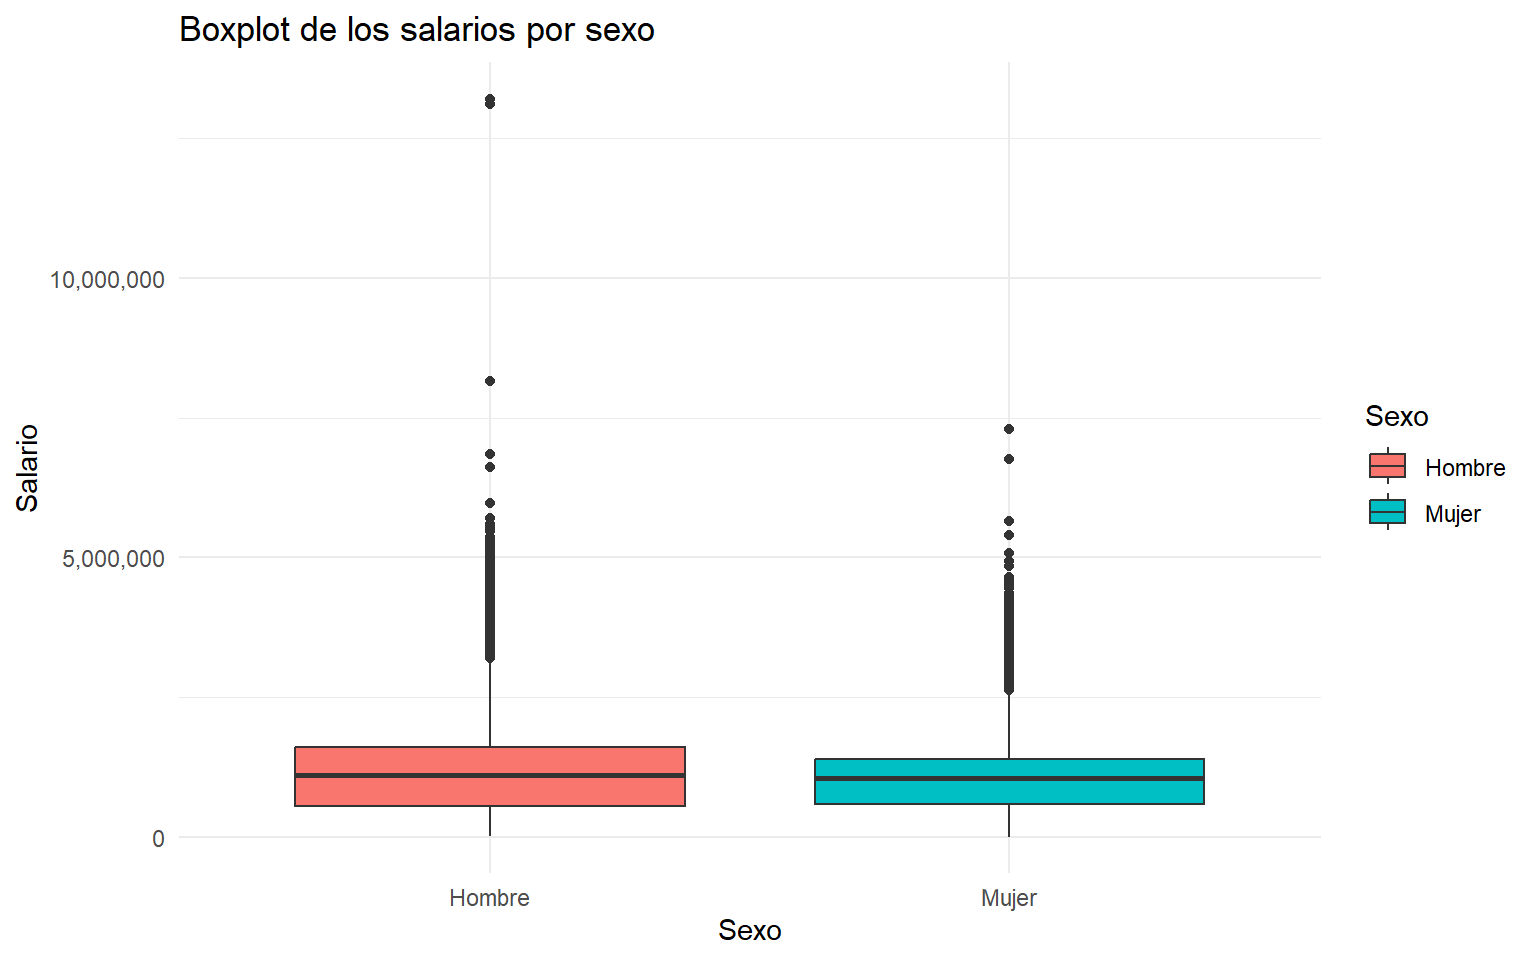
\includegraphics{Tarea_1_estadística_ii_files/figure-latex/unnamed-chunk-3-1.pdf}

\textbf{3.¿Qué puede concluir con respecto a los salarios y sexo?
¿Existe alguna diferencia entre los sexos a nivel salarial?}

De acuerdo con el gráfico de caja de bigotes, se muestra que los hombres
presentan un salario central superior al de las mujeres. También, para
el caso de las mujeres, la mediana está más cercana a la parte superior
de la caja lo que indica un sesgo a la izquierda, lo que significa que
la media es inferior a la mediana. En cuanto a los hombres,
prácticamente no se muestra sesgo, ya que, la mediana se muestra muy
centrada lo que indica una mayor simetría. Además, es posible ver que el
salario máximo de los hombres es significativamente superior al de las
mujeres estando por encima de los diez millones de colones, en cambio,
el mayor salario para una mujer es de 7 290 150. Para los hombres, la
varianza se muestra casi el doble que el de las mujeres, lo cual, se
puede explicar mediante lo descrito anteriormente. Esto indica que
existen diferencias según el sexo en cuanto a salarios.

\textbf{4.Compare su conclusión con una prueba de hipótesis sobre las
medias de las categorías de sexo.}

Se aplica la prueba t.test para comparar las medias de los salarios de
los hombres y mujeres con el fin de encontrar diferencias o no entre los
salarios y corroborar la conclusión del inciso anterior. Para la
aplicación de la prueba se considera como hipótesis nula que la
diferencia entre las medias es de cero. Además, se emplea un nivel de
significancia del 5\%. Los resultados obtenidos son los siguientes:

\begin{Shaded}
\begin{Highlighting}[]
\NormalTok{salarios\_hombres }\OtherTok{\textless{}{-}}\FunctionTok{split}\NormalTok{(BD, BD}\SpecialCharTok{$}\NormalTok{Sexo)[[}\DecValTok{1}\NormalTok{]][[}\DecValTok{5}\NormalTok{]]}
\NormalTok{salarios\_mujeres }\OtherTok{\textless{}{-}} \FunctionTok{split}\NormalTok{(BD, BD}\SpecialCharTok{$}\NormalTok{Sexo)[[}\DecValTok{2}\NormalTok{]][[}\DecValTok{5}\NormalTok{]]}

\FunctionTok{t.test}\NormalTok{(salarios\_hombres, salarios\_mujeres)}
\end{Highlighting}
\end{Shaded}

\begin{verbatim}
## 
##  Welch Two Sample t-test
## 
## data:  salarios_hombres and salarios_mujeres
## t = 25.046, df = 49886, p-value < 2.2e-16
## alternative hypothesis: true difference in means is not equal to 0
## 95 percent confidence interval:
##  101889.5 119190.8
## sample estimates:
## mean of x mean of y 
##   1157202   1046661
\end{verbatim}

Como se indica, el p-valor de la prueba es menor a 2.2e-16, esto implica
que la hipótesis nula es rechazada. Por ende, se acepta con un nivel de
confianza del 95\% que existe diferencias entre los salarios promedios
de hombres y mujeres. Por tanto, se obtiene la misma conclusión que el
inciso anterior.

\hypertarget{parte-ii}{%
\section{Parte II}\label{parte-ii}}

\textbf{Utilizando la variable U.Salarios sin filtrar por Sexo,
construya:}

\textbf{1. El histograma de los salarios.}

Antes de realizar el histograma se deciden eliminar los outliers más
distantes para que esto no afecte a la hora de graficar. Los eliminados
son aquellos salarios superiores a los 10 millones de colones, esto
debido a que son valores muy altos que se alejan de manera muy
significativa del promedio. En total fueron eliminadas dos
observaciones.

\begin{Shaded}
\begin{Highlighting}[]
\NormalTok{BD }\OtherTok{\textless{}{-}}\NormalTok{ BD[BD}\SpecialCharTok{$}\NormalTok{Salario }\SpecialCharTok{\textless{}=} \DecValTok{10000000}\NormalTok{, ]}
\end{Highlighting}
\end{Shaded}

Después de tener la base de datos adecuada, se realiza el histograma de
los salarios.

\begin{Shaded}
\begin{Highlighting}[]
\CommentTok{\#Histograma de los salarios }
\NormalTok{hist\_salarios }\OtherTok{\textless{}{-}} \FunctionTok{ggplot}\NormalTok{(BD, }\FunctionTok{aes}\NormalTok{(}\AttributeTok{x =}\NormalTok{ Salario)) }\SpecialCharTok{+}
  \FunctionTok{geom\_histogram}\NormalTok{(}\AttributeTok{fill =} \StringTok{"lightblue"}\NormalTok{, }\AttributeTok{color =} \StringTok{"black"}\NormalTok{, }\AttributeTok{alpha =} \FloatTok{0.7}\NormalTok{) }\SpecialCharTok{+}
  \FunctionTok{labs}\NormalTok{(}\AttributeTok{title =} \StringTok{"Histograma de Salarios"}\NormalTok{, }\AttributeTok{x =} \StringTok{"Salario"}\NormalTok{, }\AttributeTok{y =} \StringTok{"Frecuencia"}\NormalTok{) }\SpecialCharTok{+} 
  \FunctionTok{scale\_x\_continuous}\NormalTok{(}\AttributeTok{labels =}\NormalTok{ scales}\SpecialCharTok{::}\FunctionTok{comma\_format}\NormalTok{()) }\SpecialCharTok{+}
  \FunctionTok{scale\_y\_continuous}\NormalTok{(}\AttributeTok{labels =}\NormalTok{ scales}\SpecialCharTok{::}\FunctionTok{comma\_format}\NormalTok{()) }\SpecialCharTok{+}
  \FunctionTok{theme\_minimal}\NormalTok{()}
\FunctionTok{print}\NormalTok{(hist\_salarios)}
\end{Highlighting}
\end{Shaded}

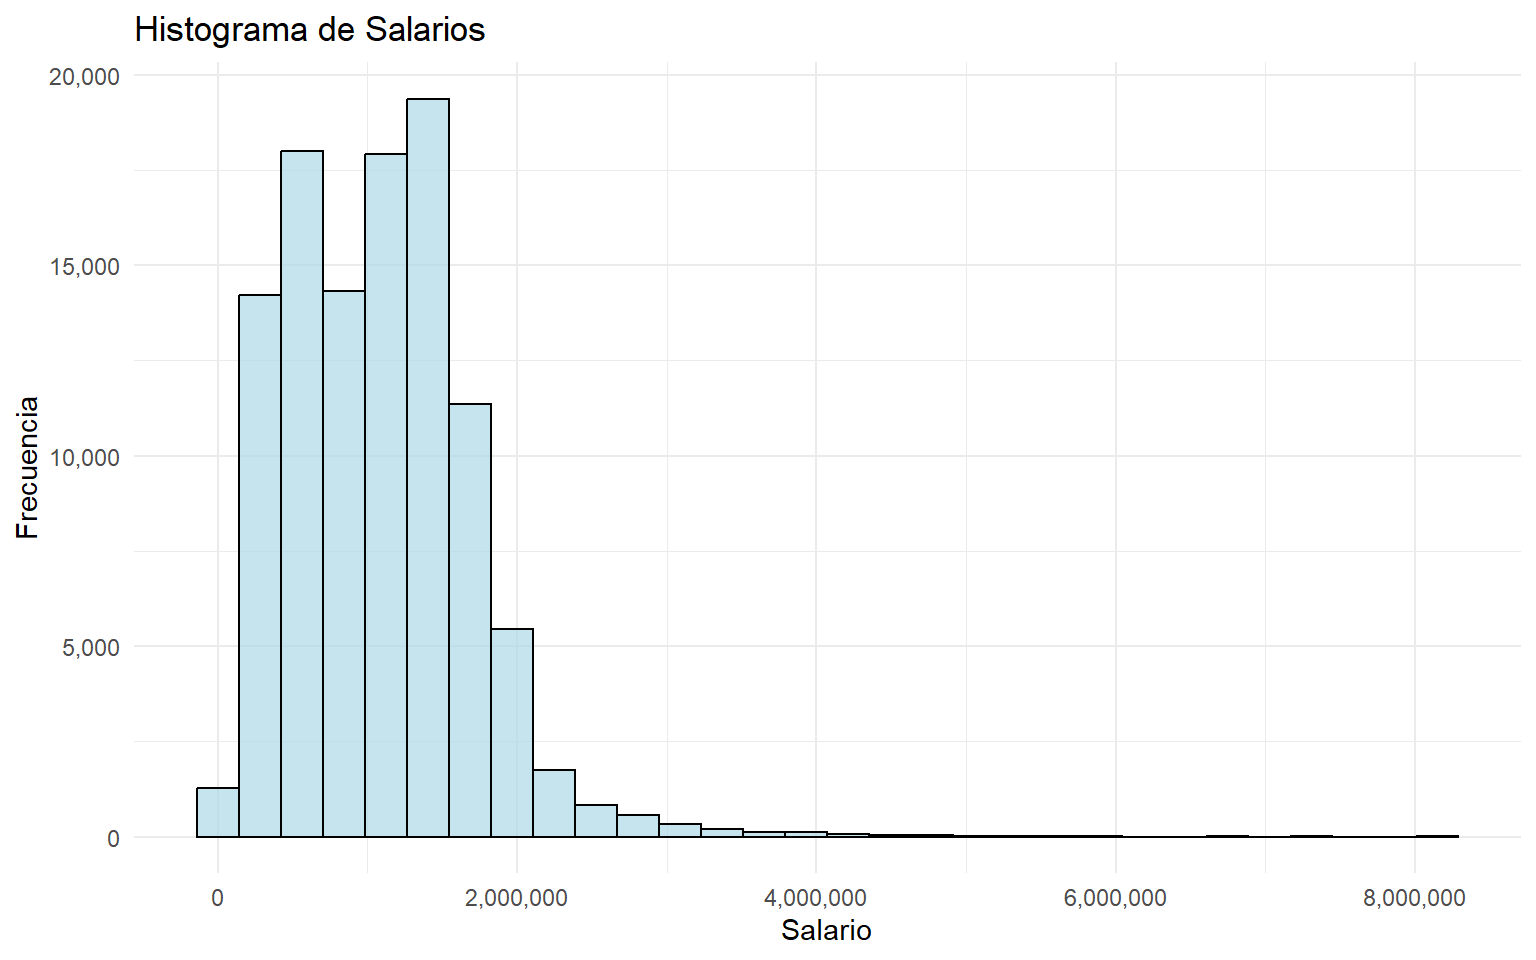
\includegraphics{Tarea_1_estadística_ii_files/figure-latex/unnamed-chunk-6-1.pdf}

\textbf{2.La densidad de los salarios por kernel (no paramétrica) usando
como kernel:}

\textbf{a.Biweigth}

\textbf{b.Normal (gaussiana)}

\textbf{c.Epanechnikov}

\textbf{d.Coseno}

\textbf{e.Uniforme (rectangular)}

\textbf{f.Triangular}

\textbf{Para todas use como bw igual al cross-validation insesgado}

Para mayor facilidad se decidió hacer una función que creara cada
gráfico por medio de la función predeterminada density. Además, se
ajustan algunos detalles del gráfico para que sea más legible.

\begin{Shaded}
\begin{Highlighting}[]
\NormalTok{Kernels }\OtherTok{\textless{}{-}} \FunctionTok{c}\NormalTok{(}\StringTok{"biweight"}\NormalTok{, }\StringTok{"gaussian"}\NormalTok{, }\StringTok{"epanechnikov"}\NormalTok{, }\StringTok{"cosine"}\NormalTok{, }\StringTok{"rectangular"}\NormalTok{, }\StringTok{"triangular"}\NormalTok{)}

\NormalTok{densidades }\OtherTok{\textless{}{-}} \FunctionTok{lapply}\NormalTok{(Kernels, }\ControlFlowTok{function}\NormalTok{(kernel) \{}
  \FunctionTok{density}\NormalTok{(BD}\SpecialCharTok{$}\NormalTok{Salario, }\AttributeTok{kernel =}\NormalTok{ kernel, }\AttributeTok{bw =} \StringTok{"ucv"}\NormalTok{)}
\NormalTok{\})}

\NormalTok{crear\_grafico\_kernel }\OtherTok{\textless{}{-}} \ControlFlowTok{function}\NormalTok{(densidad, titulo, col) \{}
  \FunctionTok{ggplot}\NormalTok{(}\FunctionTok{data.frame}\NormalTok{(}\AttributeTok{x =}\NormalTok{ densidad}\SpecialCharTok{$}\NormalTok{x, }\AttributeTok{y =}\NormalTok{ densidad}\SpecialCharTok{$}\NormalTok{y), }\FunctionTok{aes}\NormalTok{(}\AttributeTok{x =}\NormalTok{ x, }\AttributeTok{y =}\NormalTok{ y)) }\SpecialCharTok{+}
    \FunctionTok{geom\_line}\NormalTok{(}\AttributeTok{color =}\NormalTok{ col, }\AttributeTok{size =} \DecValTok{1}\NormalTok{) }\SpecialCharTok{+}
    \FunctionTok{labs}\NormalTok{(}\AttributeTok{title =}\NormalTok{ titulo, }\AttributeTok{y =} \StringTok{"Densidad"}\NormalTok{, }\AttributeTok{x =} \StringTok{"Salario"}\NormalTok{) }\SpecialCharTok{+}
    \FunctionTok{scale\_x\_continuous}\NormalTok{(}\AttributeTok{labels =}\NormalTok{ scales}\SpecialCharTok{::}\FunctionTok{comma\_format}\NormalTok{()) }\SpecialCharTok{+}
    \FunctionTok{scale\_y\_continuous}\NormalTok{(}\AttributeTok{labels =}\NormalTok{ scales}\SpecialCharTok{::}\FunctionTok{comma\_format}\NormalTok{()) }\SpecialCharTok{+}
    \FunctionTok{theme\_minimal}\NormalTok{()}
\NormalTok{\}}

\CommentTok{\# Límites de los ejes y cuadrícula para todos los gráficos}
\NormalTok{xlim }\OtherTok{\textless{}{-}} \FunctionTok{c}\NormalTok{(}\DecValTok{0}\NormalTok{, }\FunctionTok{max}\NormalTok{(BD}\SpecialCharTok{$}\NormalTok{Salario))}
\NormalTok{ylim }\OtherTok{\textless{}{-}} \FunctionTok{c}\NormalTok{(}\DecValTok{0}\NormalTok{, }\FunctionTok{max}\NormalTok{(}\FunctionTok{sapply}\NormalTok{(densidades, }\ControlFlowTok{function}\NormalTok{(d) }\FunctionTok{max}\NormalTok{(d}\SpecialCharTok{$}\NormalTok{y))))}
\end{Highlighting}
\end{Shaded}

A continuación se muestran los gráficos correspondientes a cada Kernel.

\begin{Shaded}
\begin{Highlighting}[]
\NormalTok{biweight }\OtherTok{\textless{}{-}} \FunctionTok{crear\_grafico\_kernel}\NormalTok{(densidades[[}\DecValTok{1}\NormalTok{]], }
                                 \StringTok{"Densidad de Salarios con Kernel Biweight"}\NormalTok{, }\StringTok{"blue"}\NormalTok{)}
\FunctionTok{print}\NormalTok{(biweight)}
\end{Highlighting}
\end{Shaded}

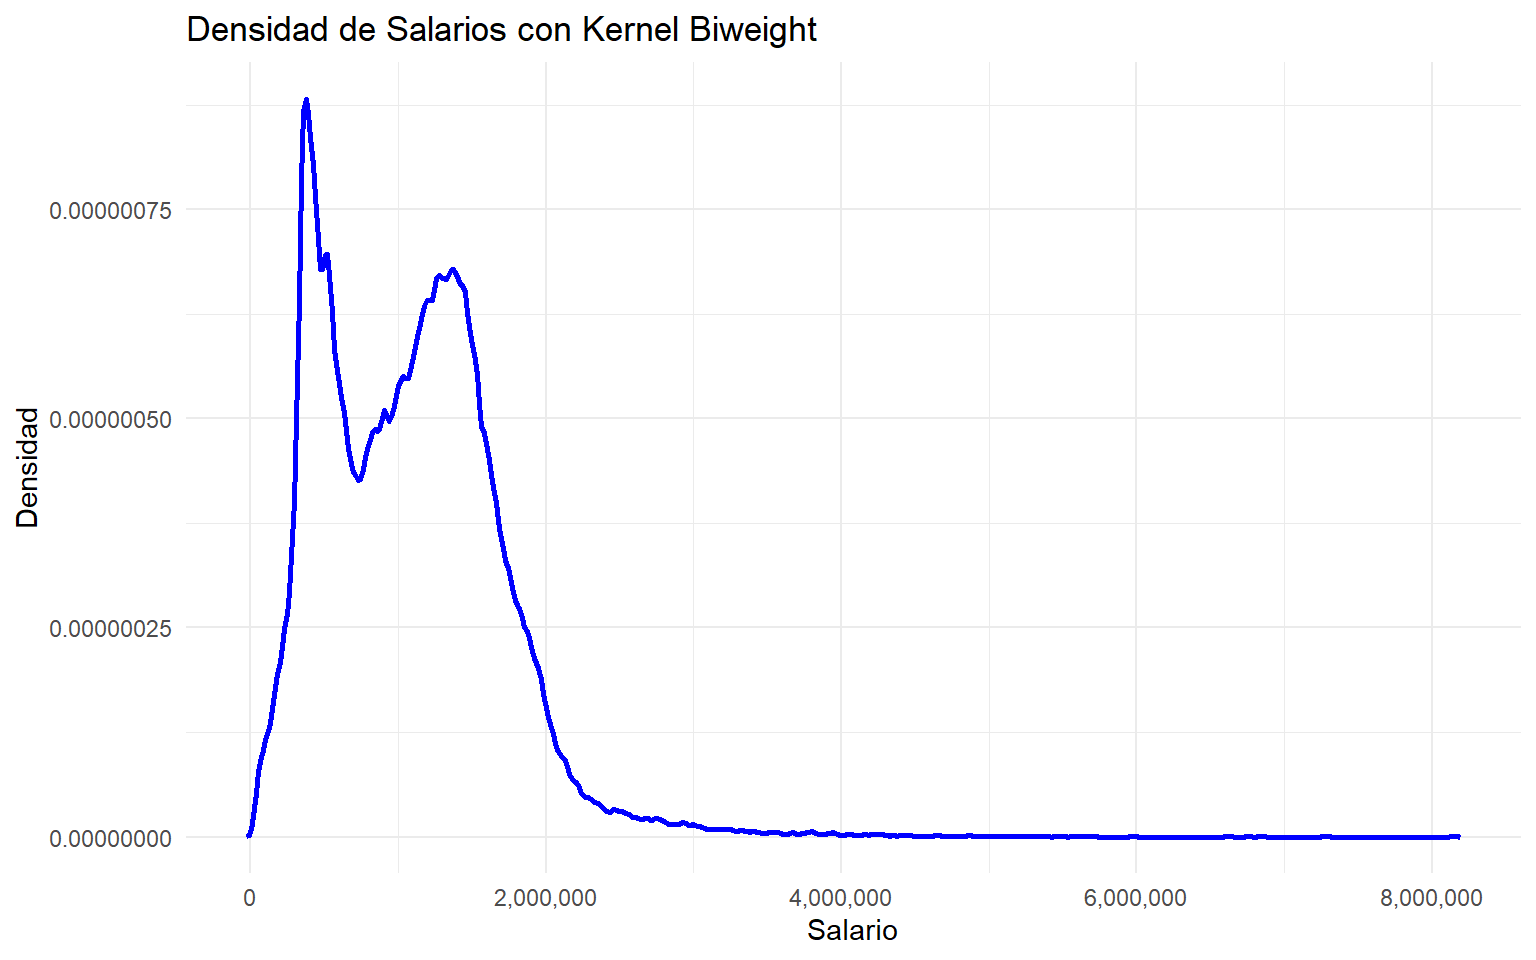
\includegraphics{Tarea_1_estadística_ii_files/figure-latex/unnamed-chunk-8-1.pdf}

\begin{Shaded}
\begin{Highlighting}[]
\NormalTok{gaussian }\OtherTok{\textless{}{-}} \FunctionTok{crear\_grafico\_kernel}\NormalTok{(densidades[[}\DecValTok{2}\NormalTok{]], }
                                 \StringTok{"Densidad de Salarios con Kernel Gaussiano"}\NormalTok{, }\StringTok{"red"}\NormalTok{)}
\FunctionTok{print}\NormalTok{(gaussian)}
\end{Highlighting}
\end{Shaded}

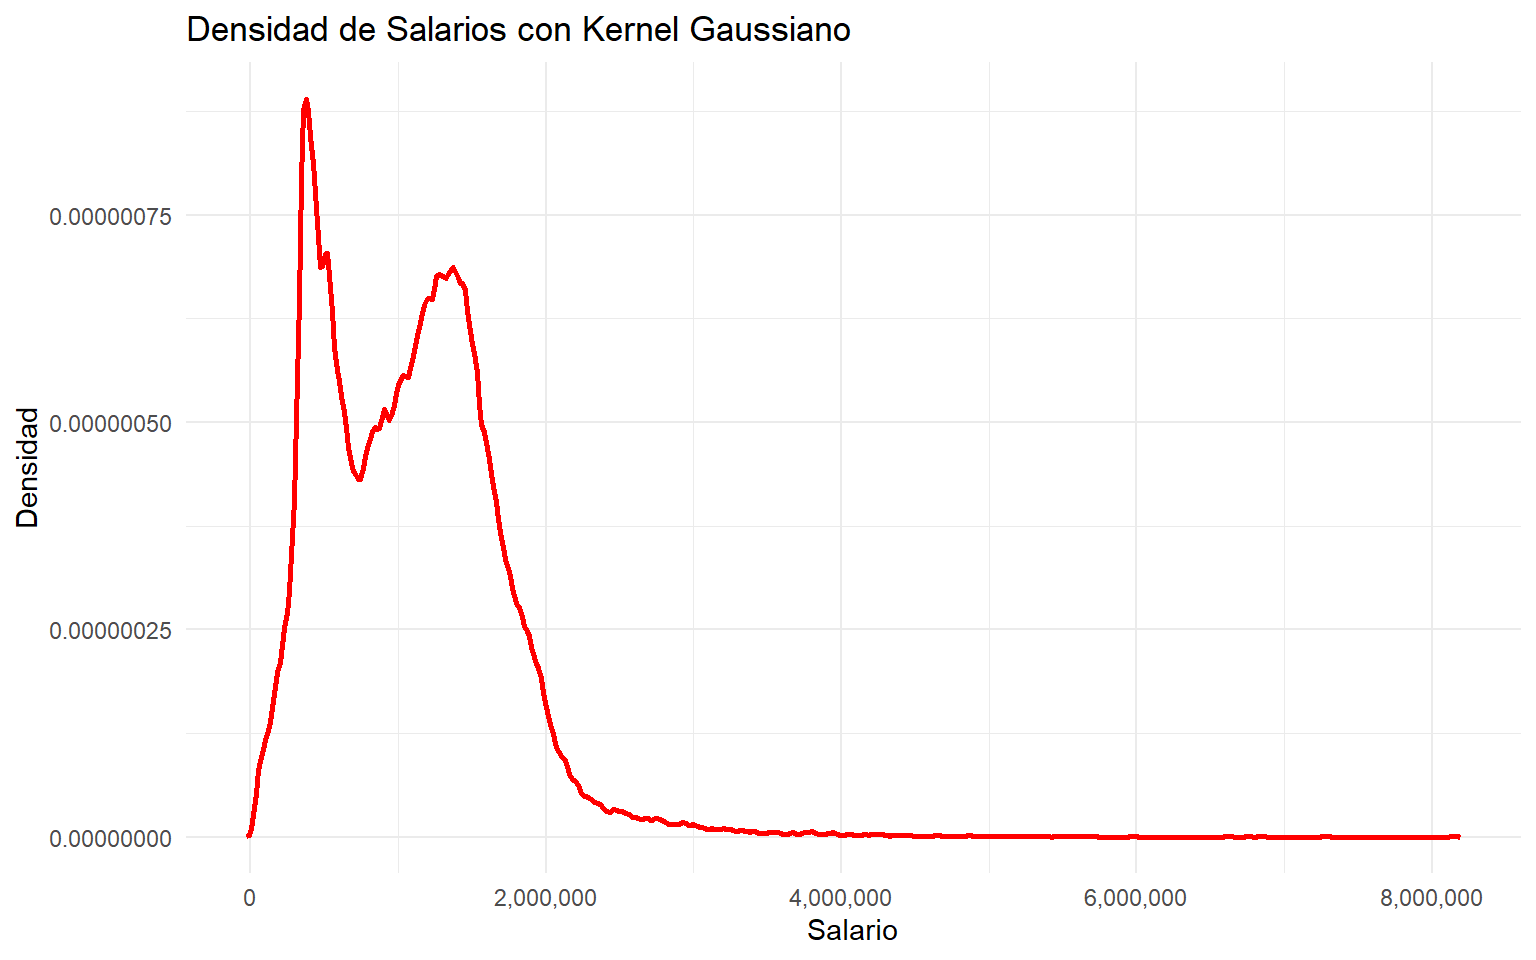
\includegraphics{Tarea_1_estadística_ii_files/figure-latex/unnamed-chunk-9-1.pdf}

\begin{Shaded}
\begin{Highlighting}[]
\NormalTok{epanechnikov }\OtherTok{\textless{}{-}} \FunctionTok{crear\_grafico\_kernel}\NormalTok{(densidades[[}\DecValTok{3}\NormalTok{]], }
                                     \StringTok{"Densidad de Salarios con Kernel Epanechnikov"}\NormalTok{,}\StringTok{"green"}\NormalTok{)}
\FunctionTok{print}\NormalTok{(epanechnikov)}
\end{Highlighting}
\end{Shaded}

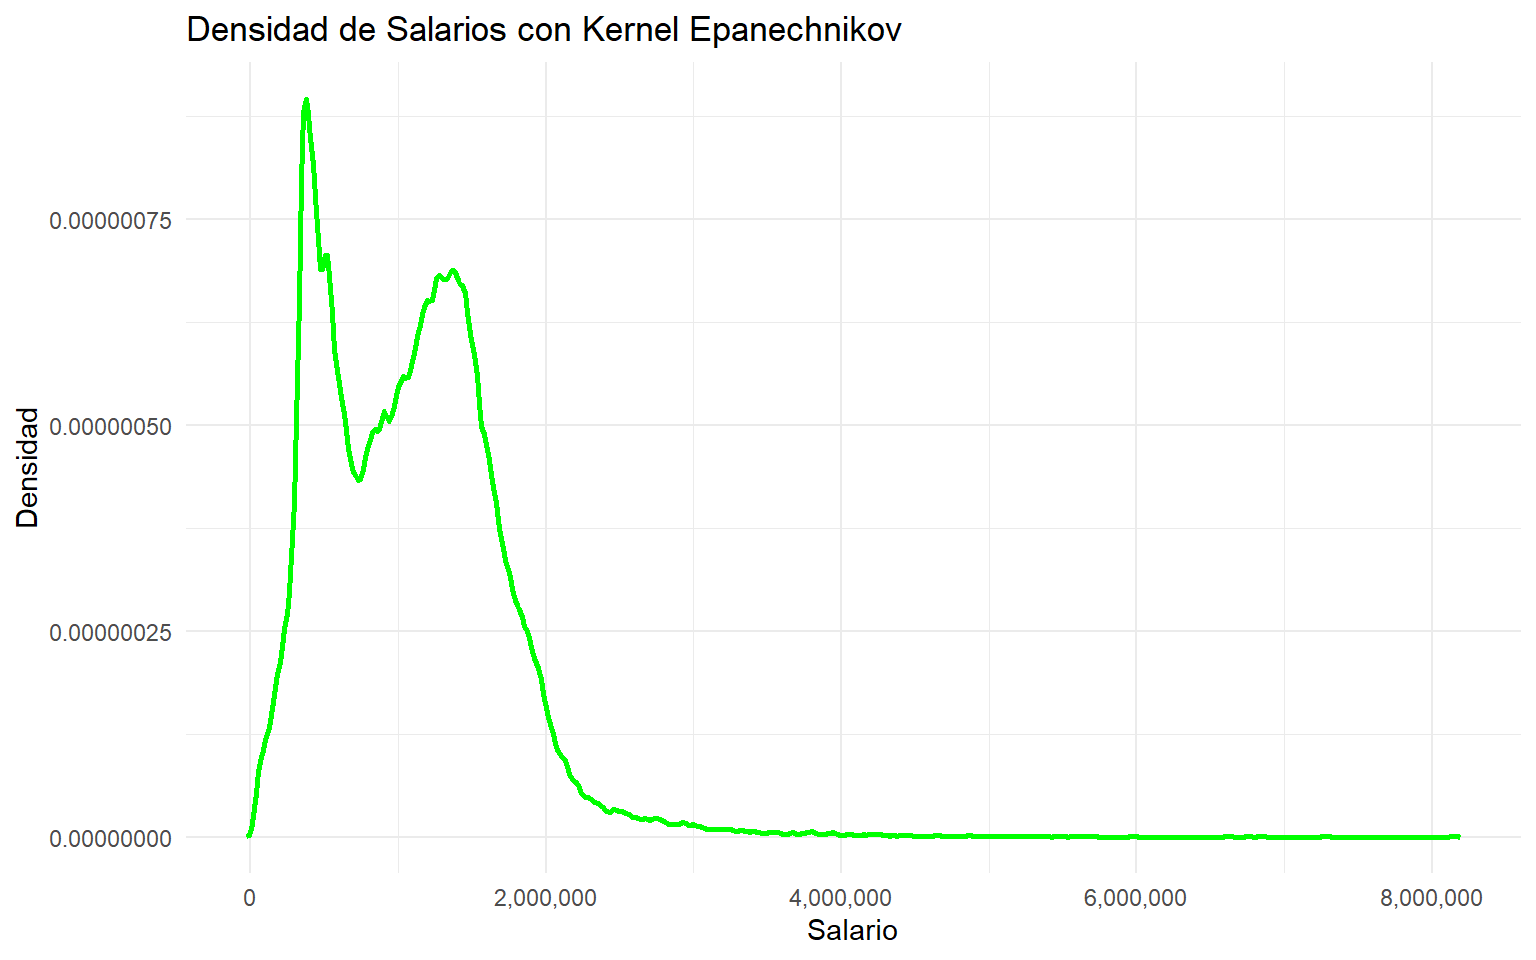
\includegraphics{Tarea_1_estadística_ii_files/figure-latex/unnamed-chunk-10-1.pdf}

\begin{Shaded}
\begin{Highlighting}[]
\NormalTok{cosine }\OtherTok{\textless{}{-}} \FunctionTok{crear\_grafico\_kernel}\NormalTok{(densidades[[}\DecValTok{4}\NormalTok{]], }
                               \StringTok{"Densidad de Salarios con Kernel Coseno"}\NormalTok{, }\StringTok{"purple"}\NormalTok{)}
\FunctionTok{print}\NormalTok{(cosine)}
\end{Highlighting}
\end{Shaded}

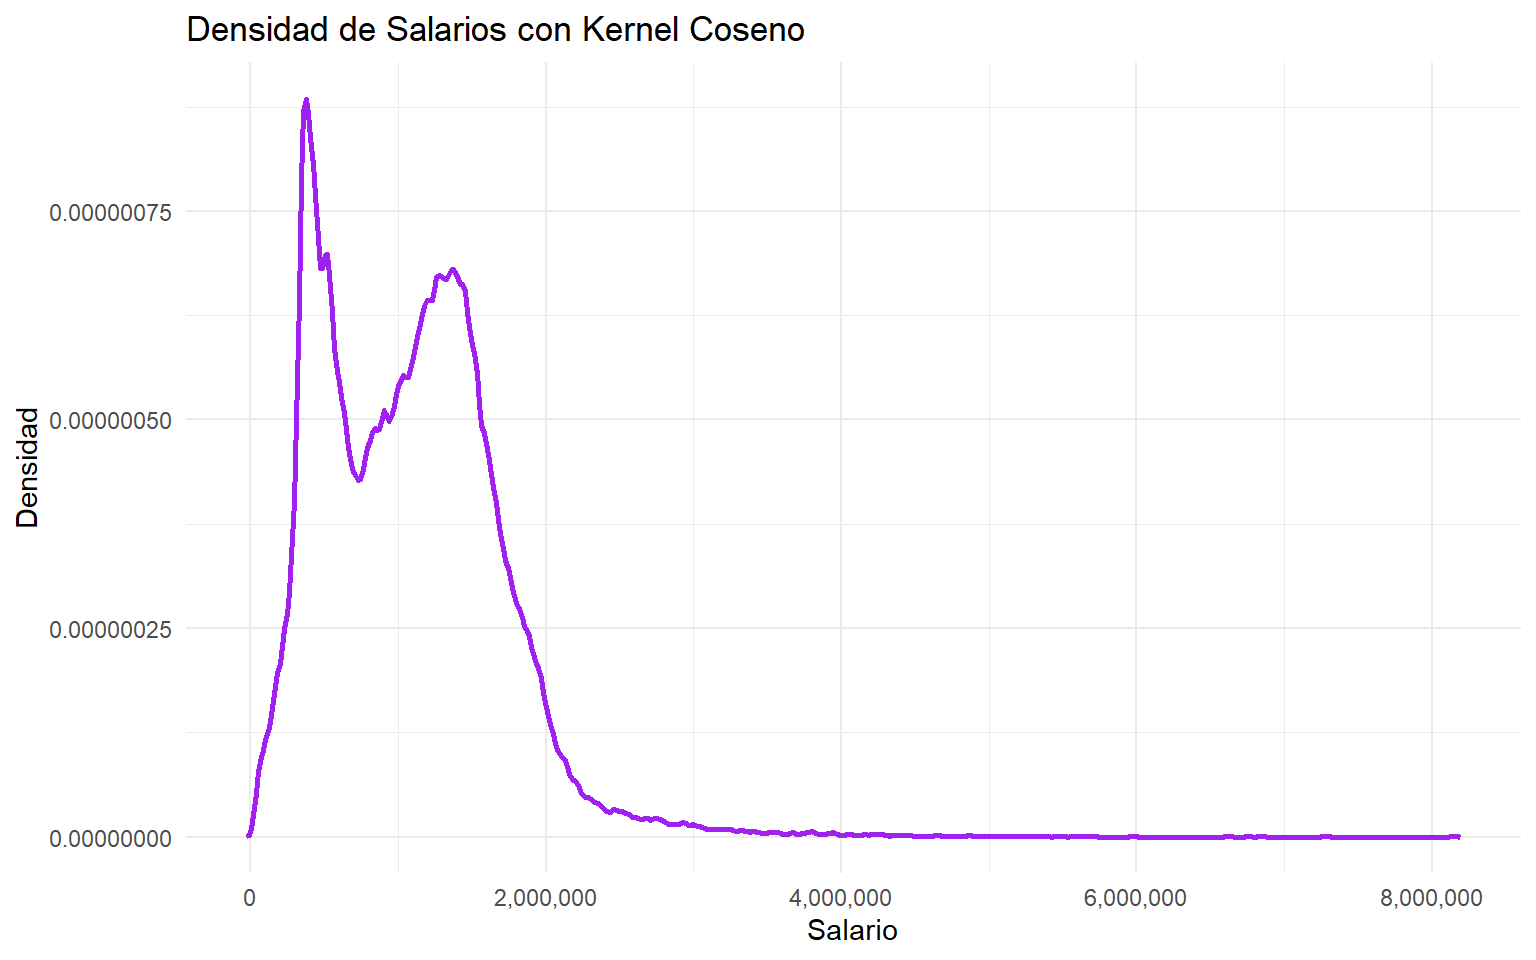
\includegraphics{Tarea_1_estadística_ii_files/figure-latex/unnamed-chunk-11-1.pdf}

\begin{Shaded}
\begin{Highlighting}[]
\NormalTok{rectangular }\OtherTok{\textless{}{-}} \FunctionTok{crear\_grafico\_kernel}\NormalTok{(densidades[[}\DecValTok{5}\NormalTok{]], }
                                    \StringTok{"Densidad de Salarios con Kernel Rectangular"}\NormalTok{, }\StringTok{"orange"}\NormalTok{)}
\FunctionTok{print}\NormalTok{(rectangular)}
\end{Highlighting}
\end{Shaded}

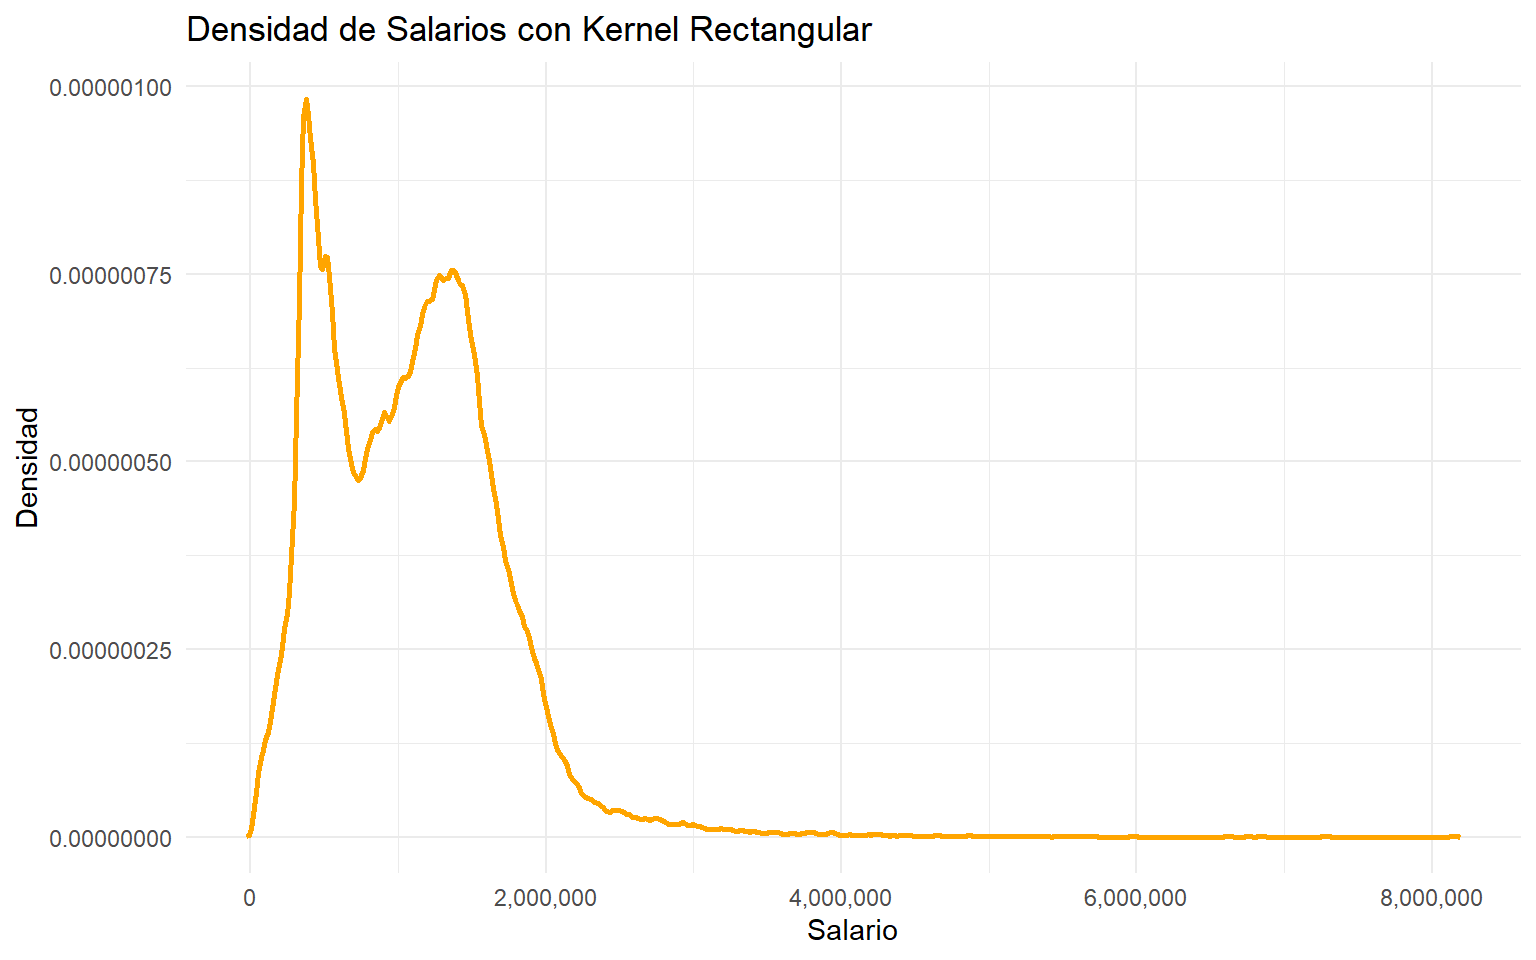
\includegraphics{Tarea_1_estadística_ii_files/figure-latex/unnamed-chunk-12-1.pdf}

\begin{Shaded}
\begin{Highlighting}[]
\NormalTok{triangular }\OtherTok{\textless{}{-}} \FunctionTok{crear\_grafico\_kernel}\NormalTok{(densidades[[}\DecValTok{6}\NormalTok{]], }
                                   \StringTok{"Densidad de Salarios con Kernel Triangular"}\NormalTok{, }\StringTok{"turquoise"}\NormalTok{)}
\FunctionTok{print}\NormalTok{(triangular)}
\end{Highlighting}
\end{Shaded}

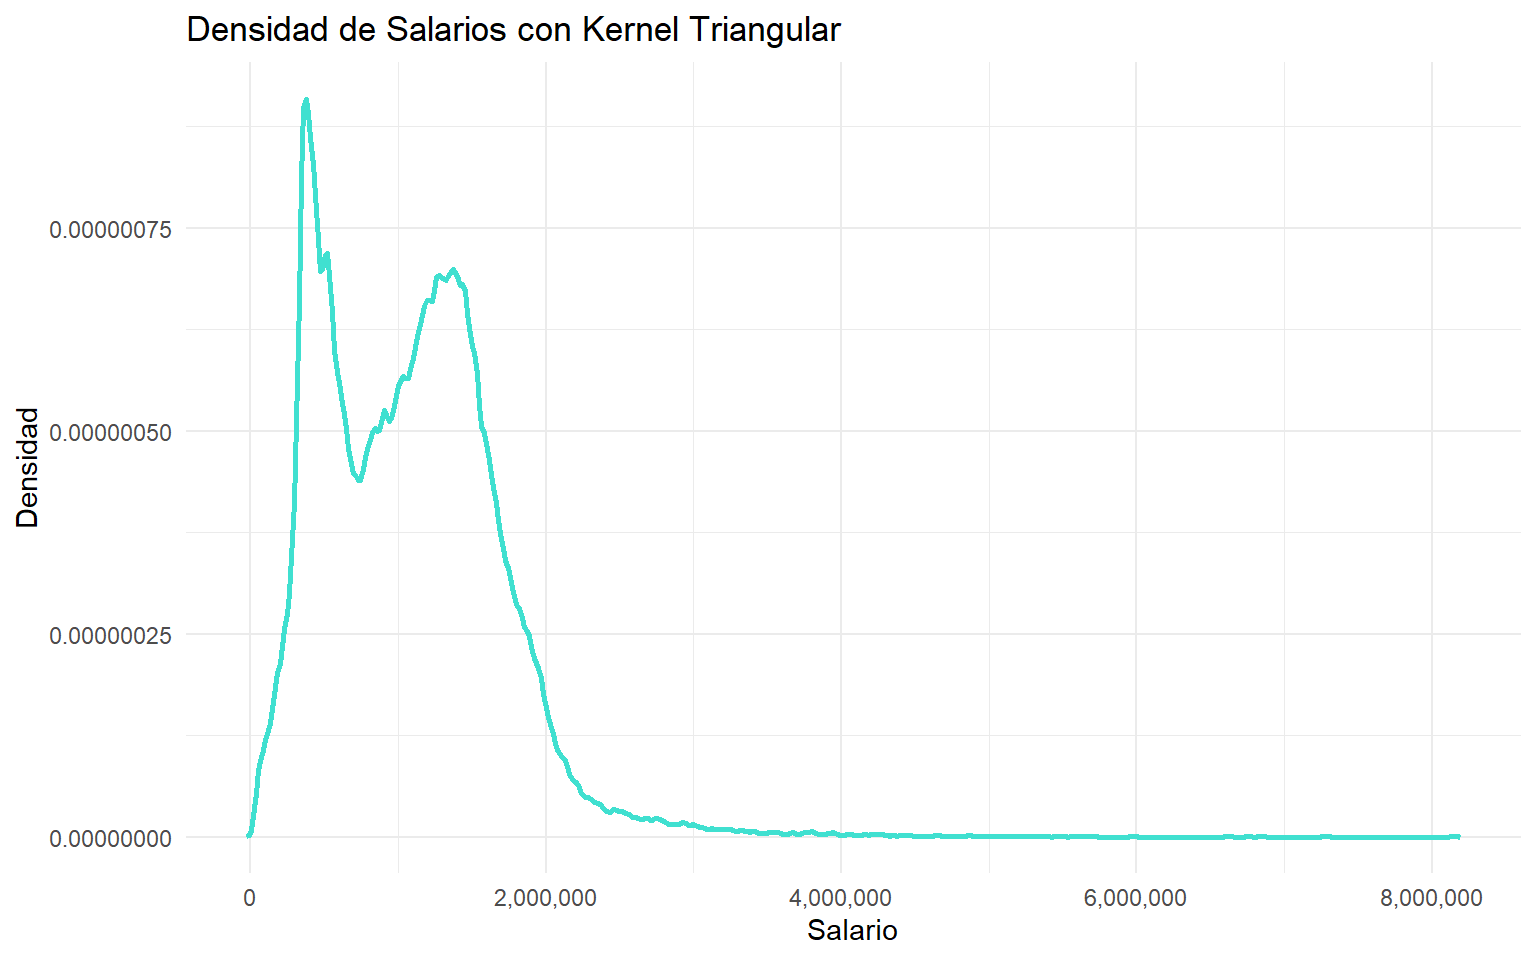
\includegraphics{Tarea_1_estadística_ii_files/figure-latex/unnamed-chunk-13-1.pdf}

\textbf{3.En un solo gráfico muestre los resultados de las densidades
con el histograma.}

Para este punto se toma el histograma del punto 1, pero se le hace un
ajuste para que no coloque la frecuencia en el eje y si no la densidad
puesto que, es lo que interesa en este caso y hace que se logre ajustar
con las curvas de densidad por kernel graficadas anteriormente.

\begin{Shaded}
\begin{Highlighting}[]
\NormalTok{hist\_salarios\_densidad }\OtherTok{\textless{}{-}} \FunctionTok{ggplot}\NormalTok{(BD, }\FunctionTok{aes}\NormalTok{(}\AttributeTok{x =}\NormalTok{ Salario, }\AttributeTok{y =} \FunctionTok{after\_stat}\NormalTok{(density))) }\SpecialCharTok{+}
  \FunctionTok{geom\_histogram}\NormalTok{(}\AttributeTok{fill =} \StringTok{"lightblue"}\NormalTok{, }\AttributeTok{color =} \StringTok{"black"}\NormalTok{, }\AttributeTok{alpha =} \FloatTok{0.7}\NormalTok{) }\SpecialCharTok{+}
  \FunctionTok{labs}\NormalTok{(}\AttributeTok{title =} \StringTok{"Histograma y Densidades de Salarios"}\NormalTok{, }\AttributeTok{x =} \StringTok{"Salario"}\NormalTok{, }\AttributeTok{y =} \StringTok{"Densidad"}\NormalTok{) }\SpecialCharTok{+} 
  \FunctionTok{scale\_x\_continuous}\NormalTok{(}\AttributeTok{labels =}\NormalTok{ scales}\SpecialCharTok{::}\FunctionTok{comma\_format}\NormalTok{()) }\SpecialCharTok{+}
  \FunctionTok{scale\_y\_continuous}\NormalTok{(}\AttributeTok{labels =}\NormalTok{ scales}\SpecialCharTok{::}\FunctionTok{comma\_format}\NormalTok{()) }\SpecialCharTok{+}
  \FunctionTok{theme\_minimal}\NormalTok{()}

\NormalTok{juntos }\OtherTok{\textless{}{-}}\NormalTok{ hist\_salarios\_densidad }\SpecialCharTok{+}
  \FunctionTok{geom\_line}\NormalTok{(}\AttributeTok{data =} \FunctionTok{data.frame}\NormalTok{(}\AttributeTok{x =}\NormalTok{ densidades[[}\DecValTok{1}\NormalTok{]]}\SpecialCharTok{$}\NormalTok{x, }\AttributeTok{y =}\NormalTok{ densidades[[}\DecValTok{1}\NormalTok{]]}\SpecialCharTok{$}\NormalTok{y, }\AttributeTok{color =}\NormalTok{ Kernels[}\DecValTok{1}\NormalTok{]), }
            \FunctionTok{aes}\NormalTok{(}\AttributeTok{x =}\NormalTok{ x, }\AttributeTok{y =}\NormalTok{ y, }\AttributeTok{color =}\NormalTok{ Kernels[}\DecValTok{1}\NormalTok{]), }\AttributeTok{size =} \DecValTok{1}\NormalTok{) }\SpecialCharTok{+}
  \FunctionTok{geom\_line}\NormalTok{(}\AttributeTok{data =} \FunctionTok{data.frame}\NormalTok{(}\AttributeTok{x =}\NormalTok{ densidades[[}\DecValTok{2}\NormalTok{]]}\SpecialCharTok{$}\NormalTok{x, }\AttributeTok{y =}\NormalTok{ densidades[[}\DecValTok{2}\NormalTok{]]}\SpecialCharTok{$}\NormalTok{y, }\AttributeTok{color =}\NormalTok{ Kernels[}\DecValTok{2}\NormalTok{]), }
            \FunctionTok{aes}\NormalTok{(}\AttributeTok{x =}\NormalTok{ x, }\AttributeTok{y =}\NormalTok{ y, }\AttributeTok{color =}\NormalTok{ Kernels[}\DecValTok{2}\NormalTok{]), }\AttributeTok{size =} \DecValTok{1}\NormalTok{) }\SpecialCharTok{+}
  \FunctionTok{geom\_line}\NormalTok{(}\AttributeTok{data =} \FunctionTok{data.frame}\NormalTok{(}\AttributeTok{x =}\NormalTok{ densidades[[}\DecValTok{3}\NormalTok{]]}\SpecialCharTok{$}\NormalTok{x, }\AttributeTok{y =}\NormalTok{ densidades[[}\DecValTok{3}\NormalTok{]]}\SpecialCharTok{$}\NormalTok{y, }\AttributeTok{color =}\NormalTok{ Kernels[}\DecValTok{3}\NormalTok{]), }
            \FunctionTok{aes}\NormalTok{(}\AttributeTok{x =}\NormalTok{ x, }\AttributeTok{y =}\NormalTok{ y, }\AttributeTok{color =}\NormalTok{ Kernels[}\DecValTok{3}\NormalTok{]), }\AttributeTok{size =} \DecValTok{1}\NormalTok{) }\SpecialCharTok{+}
  \FunctionTok{geom\_line}\NormalTok{(}\AttributeTok{data =} \FunctionTok{data.frame}\NormalTok{(}\AttributeTok{x =}\NormalTok{ densidades[[}\DecValTok{4}\NormalTok{]]}\SpecialCharTok{$}\NormalTok{x, }\AttributeTok{y =}\NormalTok{ densidades[[}\DecValTok{4}\NormalTok{]]}\SpecialCharTok{$}\NormalTok{y, }\AttributeTok{color =}\NormalTok{ Kernels[}\DecValTok{4}\NormalTok{]), }
            \FunctionTok{aes}\NormalTok{(}\AttributeTok{x =}\NormalTok{ x, }\AttributeTok{y =}\NormalTok{ y, }\AttributeTok{color =}\NormalTok{ Kernels[}\DecValTok{4}\NormalTok{]), }\AttributeTok{size =} \DecValTok{1}\NormalTok{) }\SpecialCharTok{+}
  \FunctionTok{geom\_line}\NormalTok{(}\AttributeTok{data =} \FunctionTok{data.frame}\NormalTok{(}\AttributeTok{x =}\NormalTok{ densidades[[}\DecValTok{5}\NormalTok{]]}\SpecialCharTok{$}\NormalTok{x, }\AttributeTok{y =}\NormalTok{ densidades[[}\DecValTok{5}\NormalTok{]]}\SpecialCharTok{$}\NormalTok{y, }\AttributeTok{color =}\NormalTok{ Kernels[}\DecValTok{5}\NormalTok{]), }
            \FunctionTok{aes}\NormalTok{(}\AttributeTok{x =}\NormalTok{ x, }\AttributeTok{y =}\NormalTok{ y, }\AttributeTok{color =}\NormalTok{ Kernels[}\DecValTok{5}\NormalTok{]), }\AttributeTok{size =} \DecValTok{1}\NormalTok{) }\SpecialCharTok{+}
  \FunctionTok{geom\_line}\NormalTok{(}\AttributeTok{data =} \FunctionTok{data.frame}\NormalTok{(}\AttributeTok{x =}\NormalTok{ densidades[[}\DecValTok{6}\NormalTok{]]}\SpecialCharTok{$}\NormalTok{x, }\AttributeTok{y =}\NormalTok{ densidades[[}\DecValTok{6}\NormalTok{]]}\SpecialCharTok{$}\NormalTok{y, }\AttributeTok{color =}\NormalTok{ Kernels[}\DecValTok{6}\NormalTok{]), }
            \FunctionTok{aes}\NormalTok{(}\AttributeTok{x =}\NormalTok{ x, }\AttributeTok{y =}\NormalTok{ y, }\AttributeTok{color =}\NormalTok{ Kernels[}\DecValTok{6}\NormalTok{]), }\AttributeTok{size =} \DecValTok{1}\NormalTok{) }\SpecialCharTok{+}
  \FunctionTok{scale\_color\_manual}\NormalTok{(}\AttributeTok{values =} \FunctionTok{c}\NormalTok{(}\StringTok{"blue"}\NormalTok{, }\StringTok{"red"}\NormalTok{, }\StringTok{"green"}\NormalTok{, }\StringTok{"purple"}\NormalTok{, }\StringTok{"orange"}\NormalTok{, }
                                \StringTok{"turquoise"}\NormalTok{), }\AttributeTok{labels =}\NormalTok{ Kernels) }\SpecialCharTok{+}
  \FunctionTok{labs}\NormalTok{(}\AttributeTok{color =} \StringTok{"Kernel"}\NormalTok{)}
\FunctionTok{print}\NormalTok{(juntos)}
\end{Highlighting}
\end{Shaded}

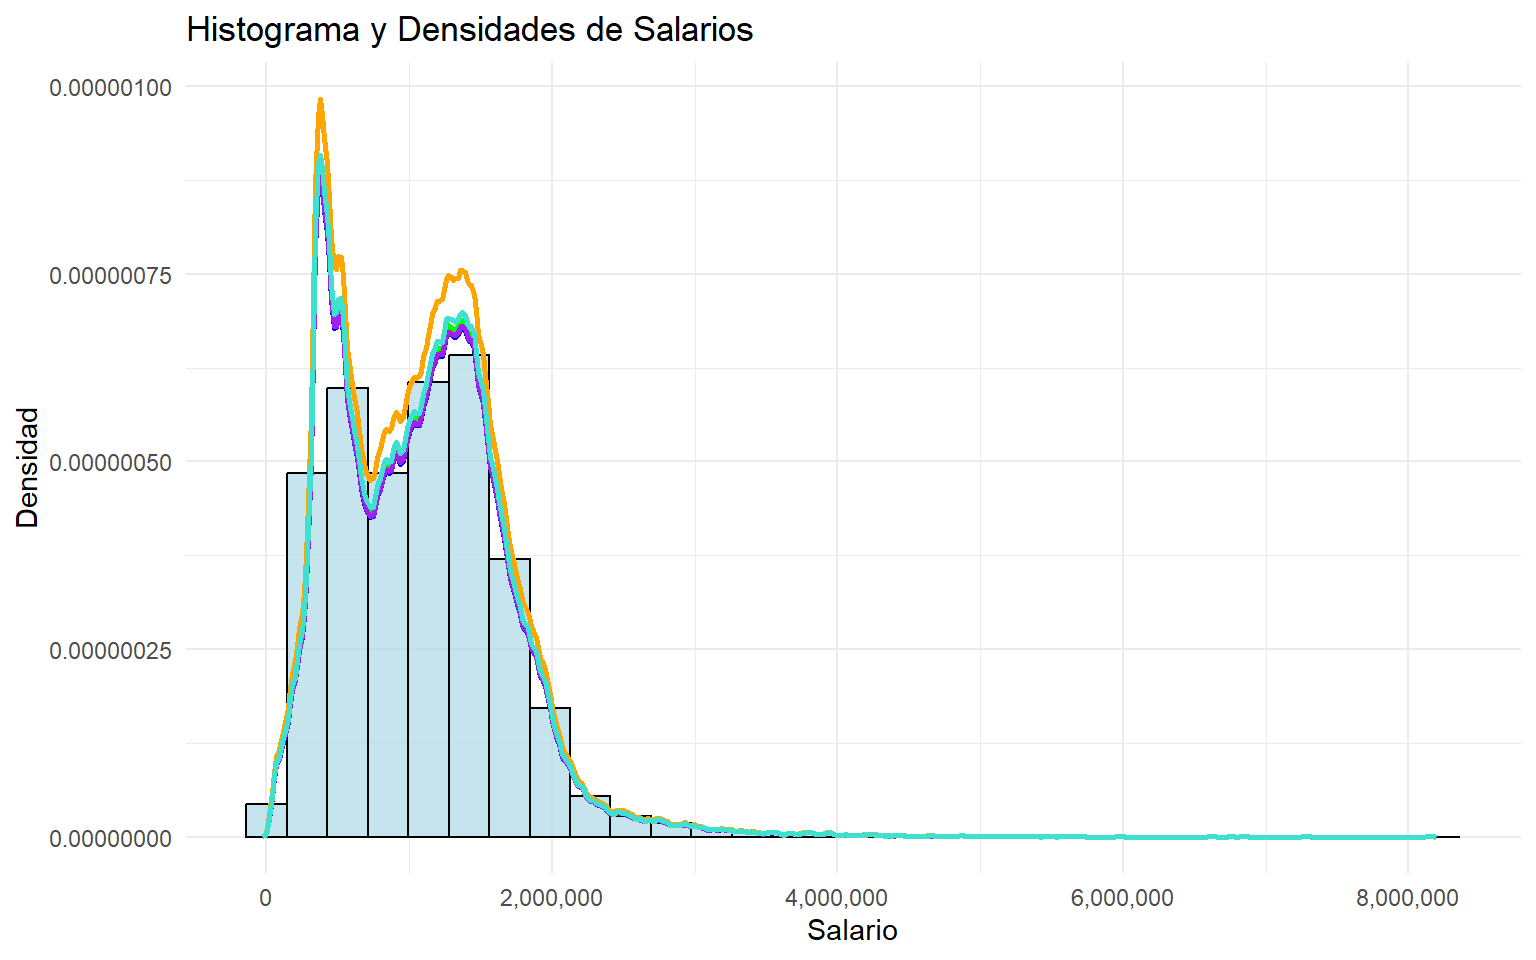
\includegraphics{Tarea_1_estadística_ii_files/figure-latex/unnamed-chunk-14-1.pdf}

\hypertarget{parte-iii}{%
\section{Parte III}\label{parte-iii}}

\textbf{1. Explique en que consiste el criterio de información de Akaike
(AIC) y cuál es el criterio de selección entre dos modelos.}

El criterio de información de Akaike (AIC) es una medida de la calidad
de un modelo dentro de un conjunto de modelos. Brinda información sobre
la complejidad de un modelo y su exactitud, pues describe el sesgo y la
varianza presentes en el modelo estadístico en estudio. Con el AIC se
permite determinar cuál modelo es el más apropiado entre los modelos
estadísticos propuestos. Como criterio de selección, se considera como
mejor modelo aquel cuyo valor de AIC es menor. Se debe tener presente
que el AIC no es prueba de hipótesis, por lo que no indica si un modelo
es de calidad, es decir, todos los modelos pueden ser erróneos y el AIC
solo indica entre ellos cúal es el que mejor se ajusta.

\textbf{2. Análisis AIC de los salarios sin filtrar por Sexo para
determinar que densidad paramétrica es la que más se le aproxima.}

A continuación, se presenta la implementación del criterio AIC mediante
la función model\_select del paquete univariateML

\begin{Shaded}
\begin{Highlighting}[]
\CommentTok{\#{-}{-}{-}{-}{-}Análisis AIC{-}{-}{-}{-}{-}|}

\CommentTok{\#Comparación densidades paramétricas por el criterio AIC}

\NormalTok{salarios }\OtherTok{\textless{}{-}}\NormalTok{ BD}\SpecialCharTok{$}\NormalTok{Salario}
\FunctionTok{model\_select}\NormalTok{(salarios, }\AttributeTok{models =}\NormalTok{ univariateML\_models, }\AttributeTok{criterion =} \StringTok{"aic"}\NormalTok{,}
             \AttributeTok{na.rm =} \ConstantTok{FALSE}\NormalTok{)}
\end{Highlighting}
\end{Shaded}

\begin{verbatim}
## Maximum likelihood estimates for the Skew Student-t model 
##      mean         sd         nu         xi  
## 1.064e+06  6.180e+05  5.387e+01  2.401e+00
\end{verbatim}

De acuerdo al resultado proporcionado, la densidad paramétrica que más
se ajusta a los datos de los salarios es la t-student.

\textbf{3. Utilizando el paquete rriskDistributions, y la función
fit.cont, bajo el criterio AIC, replique el punto 2 de esta parte.}

Empleando la función sugerida se obtiene lo siguiente:

\begin{Shaded}
\begin{Highlighting}[]
\FunctionTok{fit.cont}\NormalTok{(salarios)}
\end{Highlighting}
\end{Shaded}

\begin{Shaded}
\begin{Highlighting}[]
\NormalTok{data }\OtherTok{\textless{}{-}} \FunctionTok{data.frame}\NormalTok{(}
  \AttributeTok{Distribucion =} \FunctionTok{c}\NormalTok{(}\StringTok{"Cauchy"}\NormalTok{, }\StringTok{"Uniform"}\NormalTok{, }\StringTok{"Lognormal"}\NormalTok{, }\StringTok{"Weibull"}\NormalTok{, }\StringTok{"F"}\NormalTok{, }\StringTok{"Student"}\NormalTok{),}
  \AttributeTok{logL =} \FunctionTok{c}\NormalTok{(}\SpecialCharTok{{-}}\FloatTok{1579406.45}\NormalTok{, }\ConstantTok{NA}\NormalTok{, }\SpecialCharTok{{-}}\FloatTok{1559929.72}\NormalTok{, }\SpecialCharTok{{-}}\FloatTok{1552303.26}\NormalTok{, }\SpecialCharTok{{-}}\FloatTok{1852800.9}\NormalTok{, }\SpecialCharTok{{-}}\FloatTok{1925112.91}\NormalTok{),}
  \AttributeTok{AIC =} \FunctionTok{c}\NormalTok{(}\FloatTok{3158816.91}\NormalTok{, }\ConstantTok{NA}\NormalTok{, }\FloatTok{3119863.45}\NormalTok{, }\FloatTok{3104610.52}\NormalTok{, }\FloatTok{3705605.8}\NormalTok{, }\FloatTok{3850227.82}\NormalTok{),}
  \AttributeTok{BIC =} \FunctionTok{c}\NormalTok{(}\FloatTok{3158836.05}\NormalTok{, }\ConstantTok{NA}\NormalTok{, }\FloatTok{3119882.59}\NormalTok{, }\FloatTok{3104629.67}\NormalTok{, }\FloatTok{3705624.94}\NormalTok{, }\FloatTok{3850237.39}\NormalTok{),}
  \AttributeTok{Chisq\_value =} \FunctionTok{c}\NormalTok{(}\FloatTok{64966.97}\NormalTok{, }\ConstantTok{Inf}\NormalTok{, }\FloatTok{35838.95}\NormalTok{, }\FloatTok{11129.72}\NormalTok{, }\FloatTok{2312033.08}\NormalTok{, }\FloatTok{4676102.55}\NormalTok{),}
  \AttributeTok{Chisq\_p =} \FunctionTok{c}\NormalTok{(}\DecValTok{0}\NormalTok{, }\DecValTok{0}\NormalTok{, }\DecValTok{0}\NormalTok{, }\DecValTok{0}\NormalTok{, }\DecValTok{0}\NormalTok{, }\DecValTok{0}\NormalTok{),}
  \AttributeTok{AD\_value =} \FunctionTok{c}\NormalTok{(}\FloatTok{2262.66}\NormalTok{, }\ConstantTok{Inf}\NormalTok{, }\FloatTok{1826.63}\NormalTok{, }\FloatTok{458.63}\NormalTok{, }\FloatTok{47820.62}\NormalTok{, }\FloatTok{94832.02}\NormalTok{),}
  \AttributeTok{H\_AD =} \FunctionTok{c}\NormalTok{(}\StringTok{"rejected"}\NormalTok{, }\ConstantTok{NA}\NormalTok{, }\StringTok{"rejected"}\NormalTok{, }\StringTok{"rejected"}\NormalTok{, }\ConstantTok{NA}\NormalTok{, }\ConstantTok{NA}\NormalTok{),}
  \AttributeTok{KS\_value =} \FunctionTok{c}\NormalTok{(}\FloatTok{0.12}\NormalTok{, }\FloatTok{0.08}\NormalTok{, }\FloatTok{0.10}\NormalTok{, }\FloatTok{0.05}\NormalTok{, }\FloatTok{0.60}\NormalTok{, }\FloatTok{0.79}\NormalTok{),}
  \AttributeTok{H\_KS =} \FunctionTok{c}\NormalTok{(}\StringTok{"rejected"}\NormalTok{, }\StringTok{"rejected"}\NormalTok{, }\StringTok{"rejected"}\NormalTok{, }\StringTok{"rejected"}\NormalTok{, }\StringTok{"rejected"}\NormalTok{, }\StringTok{"rejected"}\NormalTok{)}
\NormalTok{)}

\NormalTok{knitr}\SpecialCharTok{::}\FunctionTok{kable}\NormalTok{(}
\NormalTok{  data,}
  \AttributeTok{format =} \StringTok{"latex"}\NormalTok{,}
  \AttributeTok{booktabs =} \ConstantTok{TRUE}\NormalTok{,}
  \AttributeTok{align =} \StringTok{\textquotesingle{}c\textquotesingle{}}\NormalTok{,}
  \AttributeTok{rotate.colnames =} \ConstantTok{TRUE}\NormalTok{,}
  \AttributeTok{longtable =} \ConstantTok{TRUE}\NormalTok{,}
  \AttributeTok{col.width =} \FunctionTok{c}\NormalTok{(}\DecValTok{1}\NormalTok{, }\DecValTok{1}\NormalTok{, }\DecValTok{1}\NormalTok{, }\DecValTok{1}\NormalTok{, }\DecValTok{1}\NormalTok{, }\DecValTok{1}\NormalTok{, }\DecValTok{1}\NormalTok{, }\DecValTok{1}\NormalTok{, }\DecValTok{1}\NormalTok{, }\DecValTok{1}\NormalTok{)}
\NormalTok{)}
\end{Highlighting}
\end{Shaded}

\begin{longtable}{cccccccccc}
\toprule
Distribucion & logL & AIC & BIC & Chisq\_value & Chisq\_p & AD\_value & H\_AD & KS\_value & H\_KS\\
\midrule
Cauchy & -1579406 & 3158817 & 3158836 & 64966.97 & 0 & 2262.66 & rejected & 0.12 & rejected\\
Uniform & NA & NA & NA & Inf & 0 & Inf & NA & 0.08 & rejected\\
Lognormal & -1559930 & 3119863 & 3119883 & 35838.95 & 0 & 1826.63 & rejected & 0.10 & rejected\\
Weibull & -1552303 & 3104611 & 3104630 & 11129.72 & 0 & 458.63 & rejected & 0.05 & rejected\\
F & -1852801 & 3705606 & 3705625 & 2312033.08 & 0 & 47820.62 & NA & 0.60 & rejected\\
\addlinespace
Student & -1925113 & 3850228 & 3850237 & 4676102.55 & 0 & 94832.02 & NA & 0.79 & rejected\\
\bottomrule
\end{longtable}

Usando el criterio AIC, la densidad Weibull es el que presenta menor
valor de esta medida. Por ende, se toma como la mejor distribución para
los salarios.

\textbf{4.Comente y compare los resultados de los puntos 2 y 3,
seleccione una distribución}

Los resultados obtenidos en los puntos 2 y 3 son distintos, con el
primer método se obtuvo que la densidad que mejor se aproxima es la
t-Student. Sin embargo, con la segunda forma se tiene que la mejor es la
densidad de Weibull. Para determinar cúal de estas distribuciones se
ajusta mejor, se procede a analizar los siguientes gráficos
comparativos:

\begin{Shaded}
\begin{Highlighting}[]
\CommentTok{\#{-}{-}{-}{-}Elegir distribución{-}{-}{-}|}

\CommentTok{\#Comparación gráfica entre la distribución weibull y la t{-}student}

\NormalTok{fw }\OtherTok{\textless{}{-}} \FunctionTok{fitdist}\NormalTok{(salarios, }\StringTok{"weibull"}\NormalTok{)}
\NormalTok{ft }\OtherTok{\textless{}{-}} \FunctionTok{fitdist}\NormalTok{(salarios, }\StringTok{"t.scaled"}\NormalTok{, }\AttributeTok{start=}\FunctionTok{list}\NormalTok{(}\AttributeTok{df=}\DecValTok{3}\NormalTok{,}\AttributeTok{mean=}\FunctionTok{mean}\NormalTok{(salarios),}\AttributeTok{sd=} \FunctionTok{sd}\NormalTok{(salarios)))}

\FunctionTok{par}\NormalTok{(}\AttributeTok{mfrow =} \FunctionTok{c}\NormalTok{(}\DecValTok{2}\NormalTok{,}\DecValTok{2}\NormalTok{))}
\NormalTok{leyenda }\OtherTok{\textless{}{-}}\FunctionTok{c}\NormalTok{(}\StringTok{"Weibull"}\NormalTok{, }\StringTok{"T{-}Student"}\NormalTok{)}

\FunctionTok{denscomp}\NormalTok{(}\FunctionTok{list}\NormalTok{(fw, ft), }\AttributeTok{legendtext =}\NormalTok{ leyenda)}
\FunctionTok{qqcomp}\NormalTok{(}\FunctionTok{list}\NormalTok{(fw, ft), }\AttributeTok{legendtext =}\NormalTok{ leyenda)}
\FunctionTok{cdfcomp}\NormalTok{(}\FunctionTok{list}\NormalTok{(fw, ft), }\AttributeTok{legendtext =}\NormalTok{ leyenda)}
\FunctionTok{ppcomp}\NormalTok{(}\FunctionTok{list}\NormalTok{(fw, ft), }\AttributeTok{legendtext =}\NormalTok{ leyenda)}
\end{Highlighting}
\end{Shaded}

\includegraphics{Tarea_1_estadística_ii_files/figure-latex/unnamed-chunk-18-1.pdf}

A partir del gráfico del histograma con las densidades teóricas, es
posible observar que la densidad representada por la línea roja es la
que mejor se ajusta al histograma de los datos de los salarios.
Entonces, para este caso, la distribución Weibull es la que mejor se
aproxima.

Con el Q-Q plot se permiten ver las diferencias entre la distribución
teórica de los datos y la empírica. La distribución t-student y weibull
se muestran similarmente ajustados aproximadamente entre los cuántiles
teóricos 0 y 2e+06. Pero, la distribución t-student representado por el
gráfico verde, se encuentra más alejado de la línea negra al inicio y al
final de esta. Por ende, la distribución Weibull se ajusta mejor.

Para el gráfico de la distribución acumulada teórica y la empírica, las
diferencias en los ajustes entre ambas distribuciones es menos evidente.
Lo mismo para el p-p plot, por lo que, a partir de estos gráficos no se
puede deducir cuál es el mejor.

Por tanto, si consideramos los primeros dos criterios, la distribución
Weibull se ajusta mejor a los datos de los salarios en estudio.

También, la función fitdist brinda información sobre la medida AIC:

\begin{Shaded}
\begin{Highlighting}[]
\FunctionTok{print}\NormalTok{(}\FunctionTok{summary}\NormalTok{(fw))}
\end{Highlighting}
\end{Shaded}

\begin{verbatim}
## Fitting of the distribution ' weibull ' by maximum likelihood 
## Parameters : 
##           estimate Std. Error
## shape 1.889217e+00          0
## scale 1.218014e+06        NaN
## Loglikelihood:  -1552303   AIC:  3104611   BIC:  3104630 
## Correlation matrix:
##       shape scale
## shape     1   NaN
## scale   NaN     1
\end{verbatim}

\begin{Shaded}
\begin{Highlighting}[]
\FunctionTok{print}\NormalTok{(}\FunctionTok{summary}\NormalTok{(ft))}
\end{Highlighting}
\end{Shaded}

\begin{verbatim}
## Fitting of the distribution ' t.scaled ' by maximum likelihood 
## Parameters : 
##          estimate Std. Error
## df   1.329545e+01      0.000
## mean 1.034088e+06        NaN
## sd   5.569787e+05    131.072
## Loglikelihood:  -1558287   AIC:  3116581   BIC:  3116610 
## Correlation matrix:
##        df mean   sd
## df      1  NaN -Inf
## mean  NaN    1  NaN
## sd   -Inf  NaN    1
\end{verbatim}

Donde Weibull presenta el menor valor AIC. Con lo cual, se confirma que
la distribución Weibull es la que mejor se ajusta.

\textbf{5.Intervalo de confianza para la media y la desviación estándar
usando la función bootstrapml}

Para obtener los intervalos de confianza se ejecuta el siguiente código:

\begin{Shaded}
\begin{Highlighting}[]
\NormalTok{densidad\_salario }\OtherTok{\textless{}{-}} \FunctionTok{mlweibull}\NormalTok{(salarios)}

\CommentTok{\#intervalo confianza media}
\FunctionTok{bootstrapml}\NormalTok{(densidad\_salario, }\AttributeTok{map =} \ControlFlowTok{function}\NormalTok{(x) x[}\DecValTok{2}\NormalTok{]}\SpecialCharTok{*}\FunctionTok{gamma}\NormalTok{(}\DecValTok{1}\SpecialCharTok{+}\NormalTok{(}\DecValTok{1}\SpecialCharTok{/}\NormalTok{x[}\DecValTok{1}\NormalTok{])))}
\end{Highlighting}
\end{Shaded}

\begin{verbatim}
##    2.5%   97.5% 
## 1077264 1084414
\end{verbatim}

\begin{Shaded}
\begin{Highlighting}[]
\CommentTok{\#intervalo confianza desviación estándar}
\FunctionTok{bootstrapml}\NormalTok{(densidad\_salario, }\AttributeTok{map =} \ControlFlowTok{function}\NormalTok{(x) }\FunctionTok{sqrt}\NormalTok{(x[}\DecValTok{2}\NormalTok{]}\SpecialCharTok{\^{}}\DecValTok{2}\SpecialCharTok{*}\NormalTok{(}\FunctionTok{gamma}\NormalTok{(}\DecValTok{1}\SpecialCharTok{+}\DecValTok{2}\SpecialCharTok{/}\NormalTok{x[}\DecValTok{1}\NormalTok{])}\SpecialCharTok{{-}}\NormalTok{(}\FunctionTok{gamma}\NormalTok{(}\DecValTok{1}\SpecialCharTok{+}\DecValTok{1}\SpecialCharTok{/}\NormalTok{x[}\DecValTok{1}\NormalTok{]))}\SpecialCharTok{\^{}}\DecValTok{2}\NormalTok{)))}
\end{Highlighting}
\end{Shaded}

\begin{verbatim}
##     2.5%    97.5% 
## 592271.6 597561.0
\end{verbatim}

Del cual, se obtiene que el intervalo de confianza al 97.5\% para la
media es {[}1077264, 1084414{]} y para la desviación estándar es
{[}592271.6, 597561.0{]}.

\hypertarget{parte-iv}{%
\section{Parte IV}\label{parte-iv}}

\textbf{1.Del paquete ks de R, describa brevemente que realiza la
función kde y realice como ejemplo un gráfico de la densidad con U.
Salarios sin filtrar por sexo.}

Inicialmente el paquete \emph{ks} de R es un paquete orientado a
suavizar datos univariados o multivariados mediante kernels. Dentro de
este paquete se encuentra la función \emph{Kernel density estimate
(kde)} la cual estima la función de densidad de probabilidad para datos
de 1 a 6 dimensiones de forma no paramétrica.

\begin{Shaded}
\begin{Highlighting}[]
\NormalTok{KDE }\OtherTok{\textless{}{-}} \FunctionTok{kde}\NormalTok{(BD}\SpecialCharTok{$}\NormalTok{Salario)}
\FunctionTok{plot}\NormalTok{(KDE, }\AttributeTok{main =} \StringTok{"Función estimada de densidad probabilística"}\NormalTok{, }\AttributeTok{ylab =} \StringTok{""}\NormalTok{, }\AttributeTok{xlab =} \StringTok{""}\NormalTok{)}
\end{Highlighting}
\end{Shaded}

\includegraphics{Tarea_1_estadística_ii_files/figure-latex/unnamed-chunk-21-1.pdf}

\textbf{2.Del paquete boot de R, describa brevemente la función boot.ci}

Este paquete contiene funciones y bases de datos para bootstrapping del
libro \emph{Bootstrap Methods and Their Application}. La función boot.ci
genera 5 tipos diferentes de intervalos de confianza no paramétricos de
dos colas iguales: Intervalos de Aproximación normal, intervalos básicos
bootstrap, intervalos bootstrap studentnizados, intervalos percentil
bootstrap e intervalos ajustados percentil bootstrap, de los cuales se
puede hacer una selección según preferencia.

\begin{Shaded}
\begin{Highlighting}[]
\NormalTok{resultado\_boot }\OtherTok{\textless{}{-}} \FunctionTok{boot}\NormalTok{(}\AttributeTok{data=}\NormalTok{BD}\SpecialCharTok{$}\NormalTok{Salario,}
                \AttributeTok{statistic=}\ControlFlowTok{function}\NormalTok{(y,indices) }\FunctionTok{mean}\NormalTok{(y[indices]),}
                \AttributeTok{R=}\DecValTok{1000}\NormalTok{)}
\end{Highlighting}
\end{Shaded}

\textbf{3.Realice un Bootstrap de la media de los U. Salarios sin
filtrar por sexo, (para esto deben crear una función que contenga
índices) utilizando la función boot.}

\textbf{a.Estime la media Bootstrap (ver la variable t) y compárela con
la media de los datos originales (ver la variable t0).}

\begin{Shaded}
\begin{Highlighting}[]
\NormalTok{media\_real }\OtherTok{\textless{}{-}}\NormalTok{ resultado\_boot}\SpecialCharTok{$}\NormalTok{t0}
\NormalTok{media\_boot }\OtherTok{\textless{}{-}} \FunctionTok{mean}\NormalTok{(resultado\_boot}\SpecialCharTok{$}\NormalTok{t)}
\NormalTok{medias\_y\_diff }\OtherTok{\textless{}{-}} \FunctionTok{data.frame}\NormalTok{(media\_real, media\_boot, media\_real}\SpecialCharTok{{-}}\NormalTok{media\_boot)}
\FunctionTok{colnames}\NormalTok{(medias\_y\_diff) }\OtherTok{\textless{}{-}} \FunctionTok{c}\NormalTok{(}\StringTok{"Media real"}\NormalTok{, }\StringTok{"Media boot"}\NormalTok{, }\StringTok{"Diferencia"}\NormalTok{)}

\FunctionTok{print}\NormalTok{(medias\_y\_diff)}
\end{Highlighting}
\end{Shaded}

\begin{verbatim}
##   Media real Media boot Diferencia
## 1    1080558    1080569  -11.21717
\end{verbatim}

\textbf{b.Realice un histograma con los resultados del Bootstrap.}
Resulta evidente que, aunque existe una diferencia en los resultados,
esta no es de gran magnitud, mostrándose así que la media obtenida
mediante el método bootstrap es una aproximación muy certera para el
caso en cuestión.

\begin{Shaded}
\begin{Highlighting}[]
\FunctionTok{hist}\NormalTok{(resultado\_boot}\SpecialCharTok{$}\NormalTok{t, }\AttributeTok{main =} \StringTok{"Histograma de medias bootstrap"}\NormalTok{, }\AttributeTok{xlab =} \StringTok{"Medias"}\NormalTok{, }\AttributeTok{ylab =} \StringTok{"Frecuencia"}\NormalTok{)}
\end{Highlighting}
\end{Shaded}

\includegraphics{Tarea_1_estadística_ii_files/figure-latex/unnamed-chunk-24-1.pdf}

\end{document}
